\section{Warehouse-scale computers}

Services offered by warehouse-scale computers need to ensure high availability, usually targeting a minimum uptime of 99.99\%, equating to one hour of downtime per year. 
Maintaining flawless operation is challenging when managing a vast array of hardware and system software components.
Therefore, WSC workloads must be crafted to gracefully handle numerous component faults, minimizing or eliminating any adverse effects on service performance and availability.

\subsection{Architecture}
While the hardware implementation of WSCs may vary considerably, the architectural organization of these systems remains relatively consistent.
\begin{figure}[H]
    \centering
    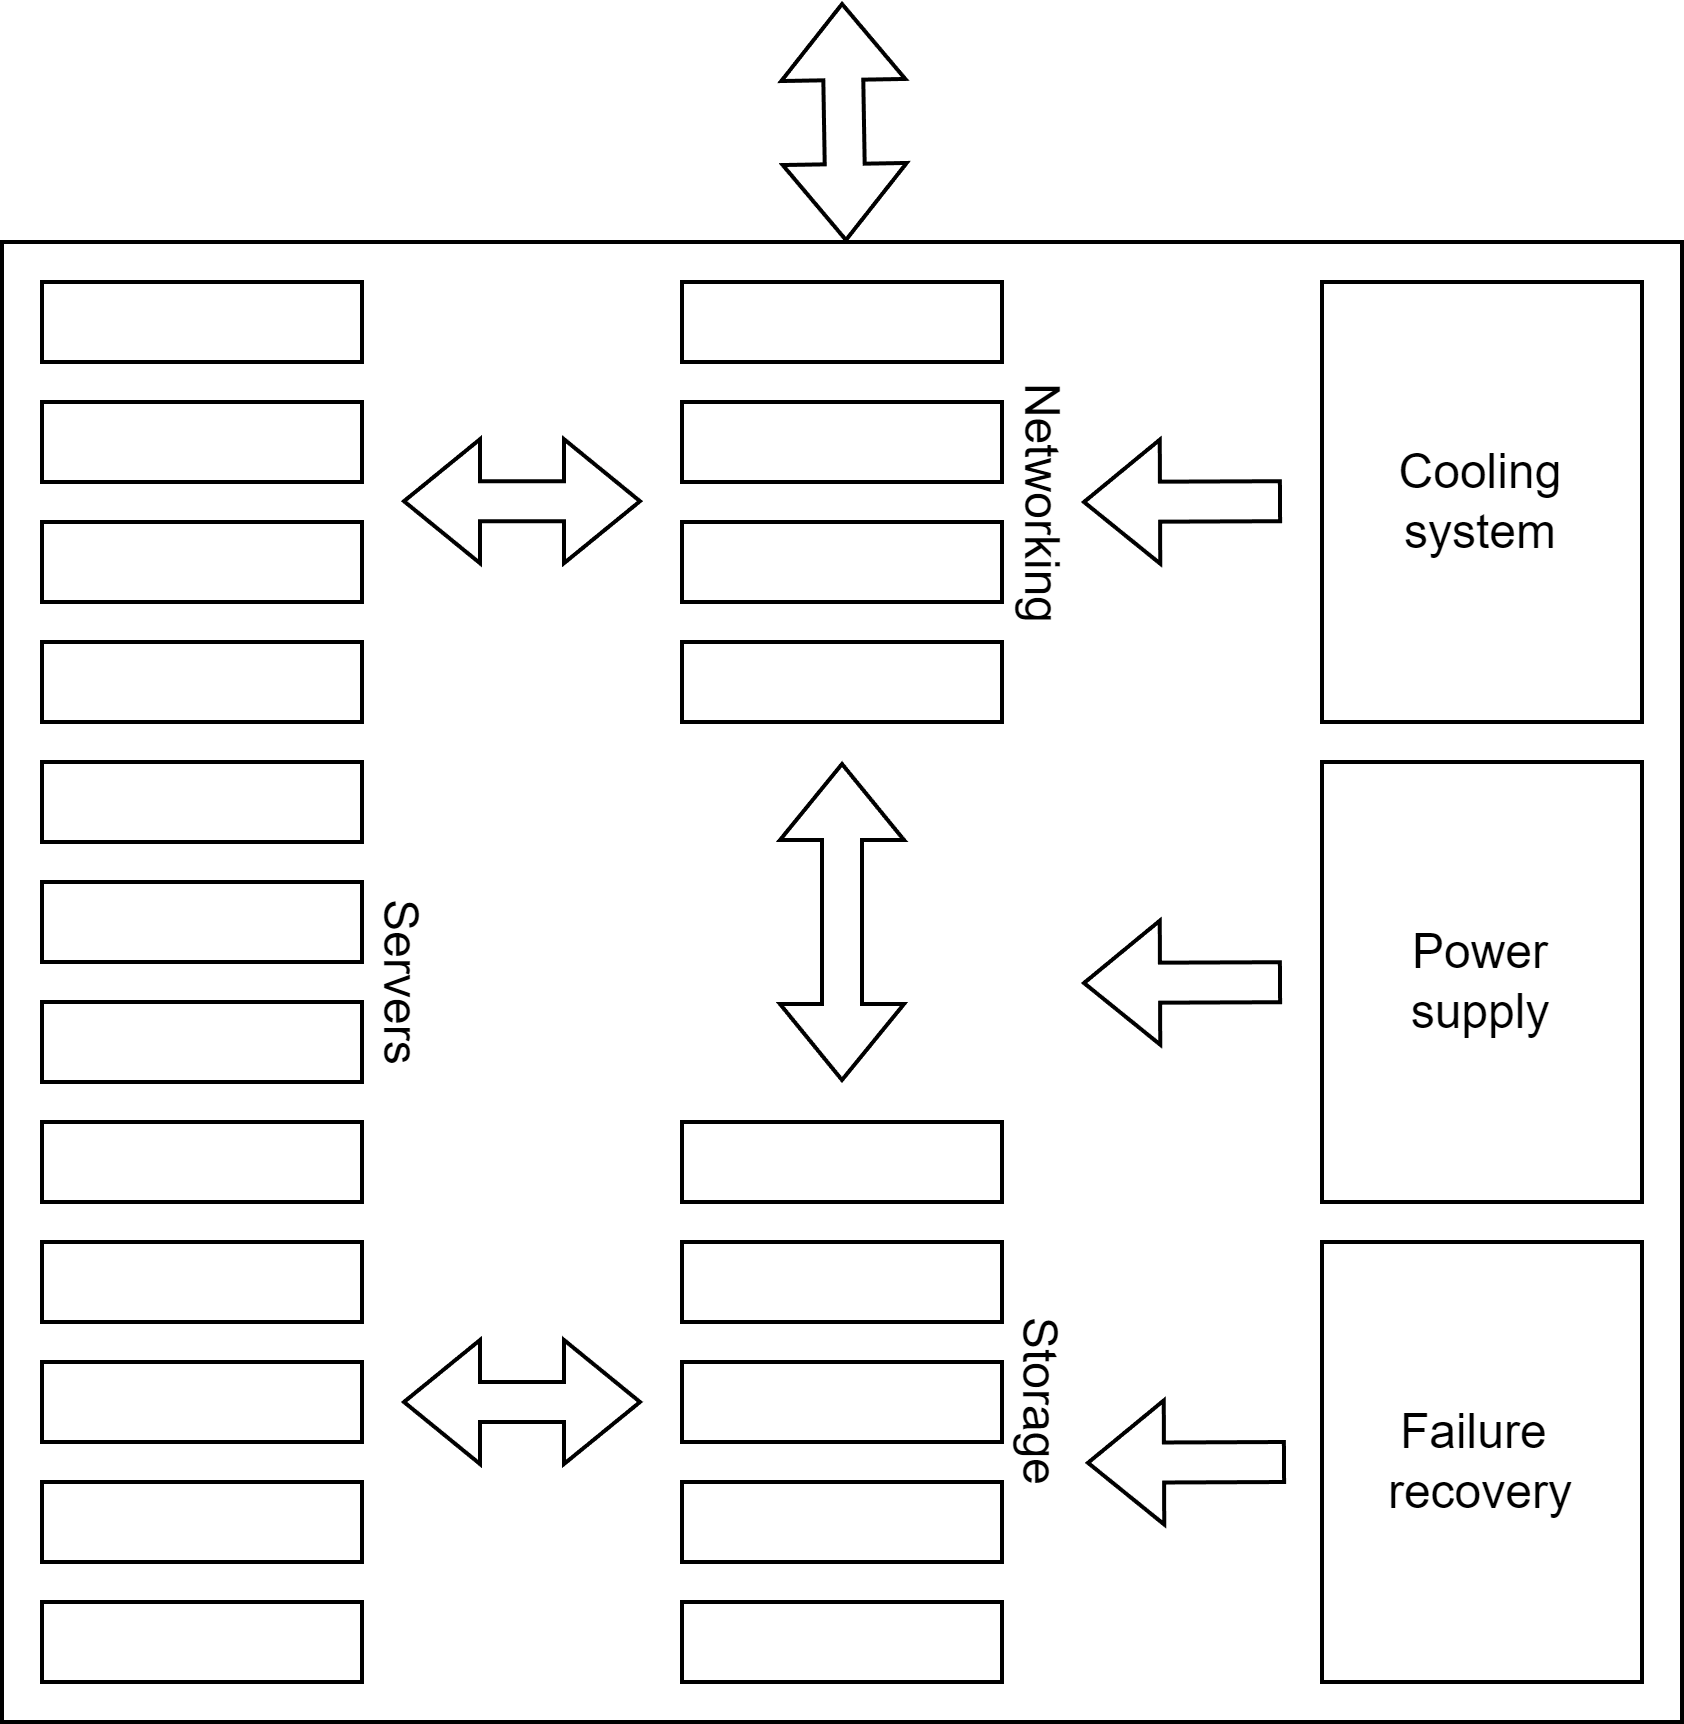
\includegraphics[width=0.5\linewidth]{images/infr.png}
    \caption{Architecture of warehouse-scale computers}
\end{figure}

\paragraph*{Servers}
Servers resemble standard PCs but are designed with form factors that enable them to fit into racks, such as rack (one or more), blade enclosure format, or tower configurations.
They can vary in terms of the number and type of CPUs, available RAM, locally attached disks (HDD, SSD, or none), as well as the inclusion of other specialized devices like GPUs, DSPs, and coprocessors.

\paragraph*{Storage}
Disks and Flash SSDs serve as the fundamental components of contemporary WSC storage systems. 
These devices are integrated into the data-center network and overseen by advanced distributed systems. 
Examples of storage configurations include Direct Attached Storage (DAS), Network Attached Storage (NAS), Storage Area Networks (SAN), and RAID controllers.

\paragraph*{Networking}
Communication equipment facilitates network interconnections among devices within the system. 
These include hubs, routers, DNS or DHCP servers, load balancers, switches, firewalls, and various other types of devices.